% \chapter*{\Huge Big Title Here}
% \addcontentsline{toc}{chapter}{Big Title Here}  % Add to TOC if needed

\chapter{Structural synergism in bovine respiratory disease modelling} % chapter title

\section{Introduction}
\subsection{Contextual background}

%-----------
%	SOUS-SOUS-SECTION 
%------------

Mathematical modelling has emerged as a cornerstone for evidence-based decision-making in animal health, increasingly recognized as indispensable by policy makers and veterinary epidemiologists  \cite{Picault2024, Ezanno2022}. Modelling frameworks offer a structured approach to understanding disease dynamics, quantifying transmission risks, forecasting outbreaks, and evaluating intervention strategies. In veterinary epidemiology, and particularly in the management of complex multi-pathogen diseases like Bovine Respiratory Disease (BRD), mathematical models serve as powerful tools that integrate knowledge across multiple disciplines, including epidemiology, veterinary science, agricultural management, and economics.

BRD is inherently complex due to its multifactorial nature, characterized by interactions between various pathogens, host susceptibility, environmental stressors, and management practices. Numerous mechanistic epidemiological models have been proposed to capture this complexity \cite{picault_modelling_2022, sorindupont_modeling_2023}. However, the mechanisms governing pathogen interactions, co-infections, and the clinical manifestations of BRD remain incompletely understood. Consequently, existing models often differ significantly in their structure, underlying assumptions, and levels of biological detail. These structural differences create uncertainties in predictions, complicating the practical task of identifying a model that accurately reflects real-world outbreak dynamics.

Recent developments emphasize the advantages of using pathogen-specific mechanistic models instead of generalized "average pathogen" approaches. Pathogens such as Orthopneumovirus bovis (BRSV), Mannheimia haemolytica (Mh), and Mycoplasmopsis bovis (Mb) exhibit distinct epidemiological characteristics, clinical progressions, and treatment responses, each requiring targeted intervention strategies. Recognizing this diversity, pathogen-specific models have been advocated for their enhanced realism and predictive accuracy in simulating BRD outbreaks. Beyond parameterization challenges, the comparative assessment of multiple valid mechanistic models necessitates addressing critical methodological dimensions. Model distinguishability, assesses whether competing models produce sufficiently distinct predictions, thereby enabling pathogen-model identification from clinical observations. Secondly, and most practically relevant, is the concept of decision impact assessment, evaluating whether the selection of a given model actually translates into measurable, economically viable, and actionable improvements on the farm. These two interconnected methodological challenges underscore the need not only for rigorously validated mechanistic models but also for frameworks capable of linking theoretical model selection directly with improved decision-making outcomes.




\subsection{Originality and objective of this work}
%-----------%-----------
%	SOUS-SECTION 
%-----------%-----------

this chapter focuses on two scientifically complementary research questions, driven by critical contextual and methodological challenges highlighted above:

\paragraph{To what extent can we reliably differentiate between multiple pathogen-specific mechanistic models of BRD, solely based on symptomatic observations ?} In this chapter, we introduce a numerical approach aimed at distinguishing among competing BRD mechanistic epidemiological models \cite{sorindupont_modeling_2023} based exclusively on observed symptomatic trajectories. Specifically, we show a general theoretical framework for pathogen-model identification, a critical issue across epidemiological contexts where accurate differentiation between pathogens is challenged by symptom overlap. The relevance of this work extends beyond Bovine Respiratory Disease (BRD), offering a broadly applicable solution for any epidemiological scenario involving multiple plausible mechanistic hypotheses or co-existing pathogens that necessitate distinct pathogen-specific management strategies. Orthopneumovirus bovis (BRSV) model captures rapid, airborne viral transmission dynamics, characterized by acute and intense infection episodes. It explicitly incorporates compartments for partial immunity, primary infection, potential reinfection (with reduced infectiousness), and rapid progression from mild to severe clinical signs, making the outbreaks swift but relatively short-lived. Mannheimia haemolytica (Mh) is modelled as an opportunistic infection primarily triggered by host immunosuppression or environmental stressors. Unlike the BRSV model, the Mh model does not account for reinfection states but includes a clear transition from asymptomatic carriage to active infection states, which can escalate into severe clinical manifestations. The infection dynamics are less explosive compared to BRSV, emphasizing progression triggered by stress-induced susceptibility. The mycoplasmosis bovis (Mb) model structurally mirrors the Mh model regarding compartments (asymptomatic carriers transitioning to symptomatic stages). However, it notably differs by emphasizing chronicity and persistence. This pathogen exhibits slower transmission, prolonged infection durations, and intermittent clinical symptom manifestation, making early detection and timely treatment more challenging and resulting in prolonged circulation within cattle populations. The probability that a treated animal recovers (for 1 dose) is set to 71\% for  Mh and 60\% for Mb. The models where calibrated using from the litterature: probabilities of recovery with antibiotic treatment (single dose) are set at 71\% for Mh and 60\% for Mb. the probability of detecting symptomatic animals (with mild clinical signs) is ... and the probability of detecting a animal displaying severe clinical signs is ...


\paragraph{Does the distinction and identification of the most likely pathogen-specific mechanistic model significantly improve practical decision-making outcomes ?} In typical cattle farming practices (conventional treatment decisions), antibiotic treatments for Bovine Respiratory Disease (BRD) are usually administered empirically based solely on observable clinical signs, without reliable pathogen identification. Under these conditions, farmers treat all symptomatic animals with antibiotics, regardless of whether the underlying infectious agent is bacterial or viral. Since antibiotics are effective only against bacteria and not viruses, this approach frequently leads to inappropriate use of antibiotics, which has two main drawbacks: if the infectious agent is viral, antibiotic treatments are unnecessary, ineffective, and economically wasteful. Such misuse increases antimicrobial resistance risks without any animal health benefit. If the infectious agent is bacterial, antibiotics are warranted and beneficial; failure to correctly administer them could lead to severe economic losses and compromised animal welfare.

To address this issue, we explicitly incorporate an economic dimension into our analysis by integrating pathogen-specific model predictions into a bio-economic framework. This enables us to quantify practical benefits, such as reductions in antibiotic usage, improved animal health outcomes, and enhanced profitability directly resulting from pathogen-informed decisions. By explicitly evaluating these consequences, our work connects theoretical epidemiological modelling with tangible, farm-level decision-making, reinforcing the practical relevance of modelling for effective livestock management.


% cite to articles discussing about cholera model distinguishability. [explain the difference between model selection and model distinguishability.]


\subsection{Main contributions and perspectives}

\subsubsection*{prognostic expert identification via model distinguishability}

Our primary methodological contribution involves numerically distinguishing three mechanistic BRD models tailored for Orthopneumovirus bovis (BRSV), Mannheimia haemolytica (Mh), and Mycoplasmopsis bovis (Mb) \cite{sorindupont_modeling_2023}. First, We constructed synthetic outbreak scenarios representative of French beef cattle farms. Three discrete-time, stochastic agent-based, pathogen-specific model  were utilized to generate outbreak trajectories over 277 days, capturing symptomatic dynamics every 12 hours for a batch of 12 calves. Variations across scenarios reflected realistic risk compositions, yielding a dataset comprising 13,650 individual simulations. Secondly, Three pathogen-specific stochastic, compartmental models \cite{sorindupont_modeling_2023} were compared, each encapsulating different transmission dynamics. Given the stochastic complexity of models and intractable likelihood functions, we employed Approximate Bayesian Computation (ABC) combined with multinomial logistic regression to identify the most likely pathogen-specific model. The ABC approach quantitatively assessed model distinguishability using summary statistics (detected symptomatic trajectories), thus allowing informed selection of the pathogen responsible for observed outbreaks.Given the stochastic complexity of models and intractable likelihood functions, we employed Approximate Bayesian Computation (ABC) combined with multinomial logistic regression to identify the most likely pathogen-specific model. The ABC approach quantitatively assessed model distinguishability using summary statistics (detected symptomatic trajectories), thus allowing informed selection of the pathogen responsible for observed outbreaks. Using synthetic symptomatic data generated under realistic farm conditions, we successfully identify the most likely pathogen-specific model with an average accuracy of approximately 93\% (fig \ref{fig:chap3-confusion-matrix}). Key performance metrics (true positive rates: BRSV=96\%, Mh=90\%, Mb=87\%) clearly indicate the feasibility and reliability of pathogen identification based on early symptomatic trajectories.

\begin{figure}[H]
  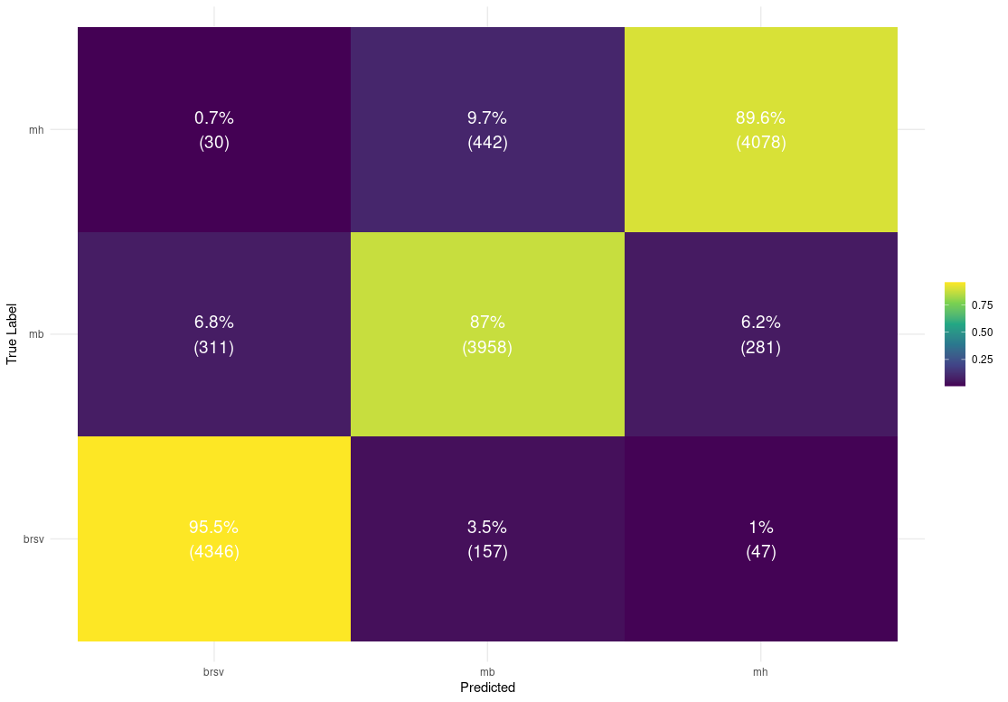
\includegraphics[width=\linewidth]{figures/chap3/chap3-confusionmatrix.png}
  \caption{Confusion matrix. Classification performance for BRSV, Mh and Mb. The diagonal represents correctly classified instances, while off-diagonal values indicate misclassification between classes.}
  \label{fig:chap3-confusion-matrix}
\end{figure}


\subsubsection*{Decision-intelligence: measuring and improving the impact on decision-making}

The second major contribution involves integrating pathogen-specific epidemiological models into a detailed economic evaluation framework. This integration enables us to quantitatively assess the economic impact of adopting pathogen-informed treatment decisions versus conventional empirical treatment strategies. Our economic model accounts explicitly for weight gain, carcass quality, feed, antibiotic treatment costs, and veterinarian interventions, calculating expected net profits and antibiotic usage for simulated cattle batches. We showed that pathogen-informed decisions substantially reduce antimicrobial use by approximately 44\% (fig \ref{fig:chap3-expectation}) in these conditions, directly addressing critical issues like antimicrobial resistance and public health safety. Simultaneously, these pathogen-informed strategies lead to a modest yet consistent increase (around 1\%) in net profitability, highlighting that economic viability can be maintained or improved even when reducing antibiotic treatments.

By leveraging the high accuracy (~93\%) of pathogen-model distinguishability, we maximize the likelihood that the correct treatment decision, either antibiotic administration for bacterial infections or withholding antibiotics for viral infections—is consistently taken.This accuracy directly improves decision-making outcomes by: Increasing the frequency of correct recommendations, thus ensuring targeted treatments that align with actual disease aetiology. And reducing incorrect or harmful decisions (false positives and false negatives), significantly decreasing inappropriate antibiotic use and associated economic and public health costs.

\begin{figure}[H]
  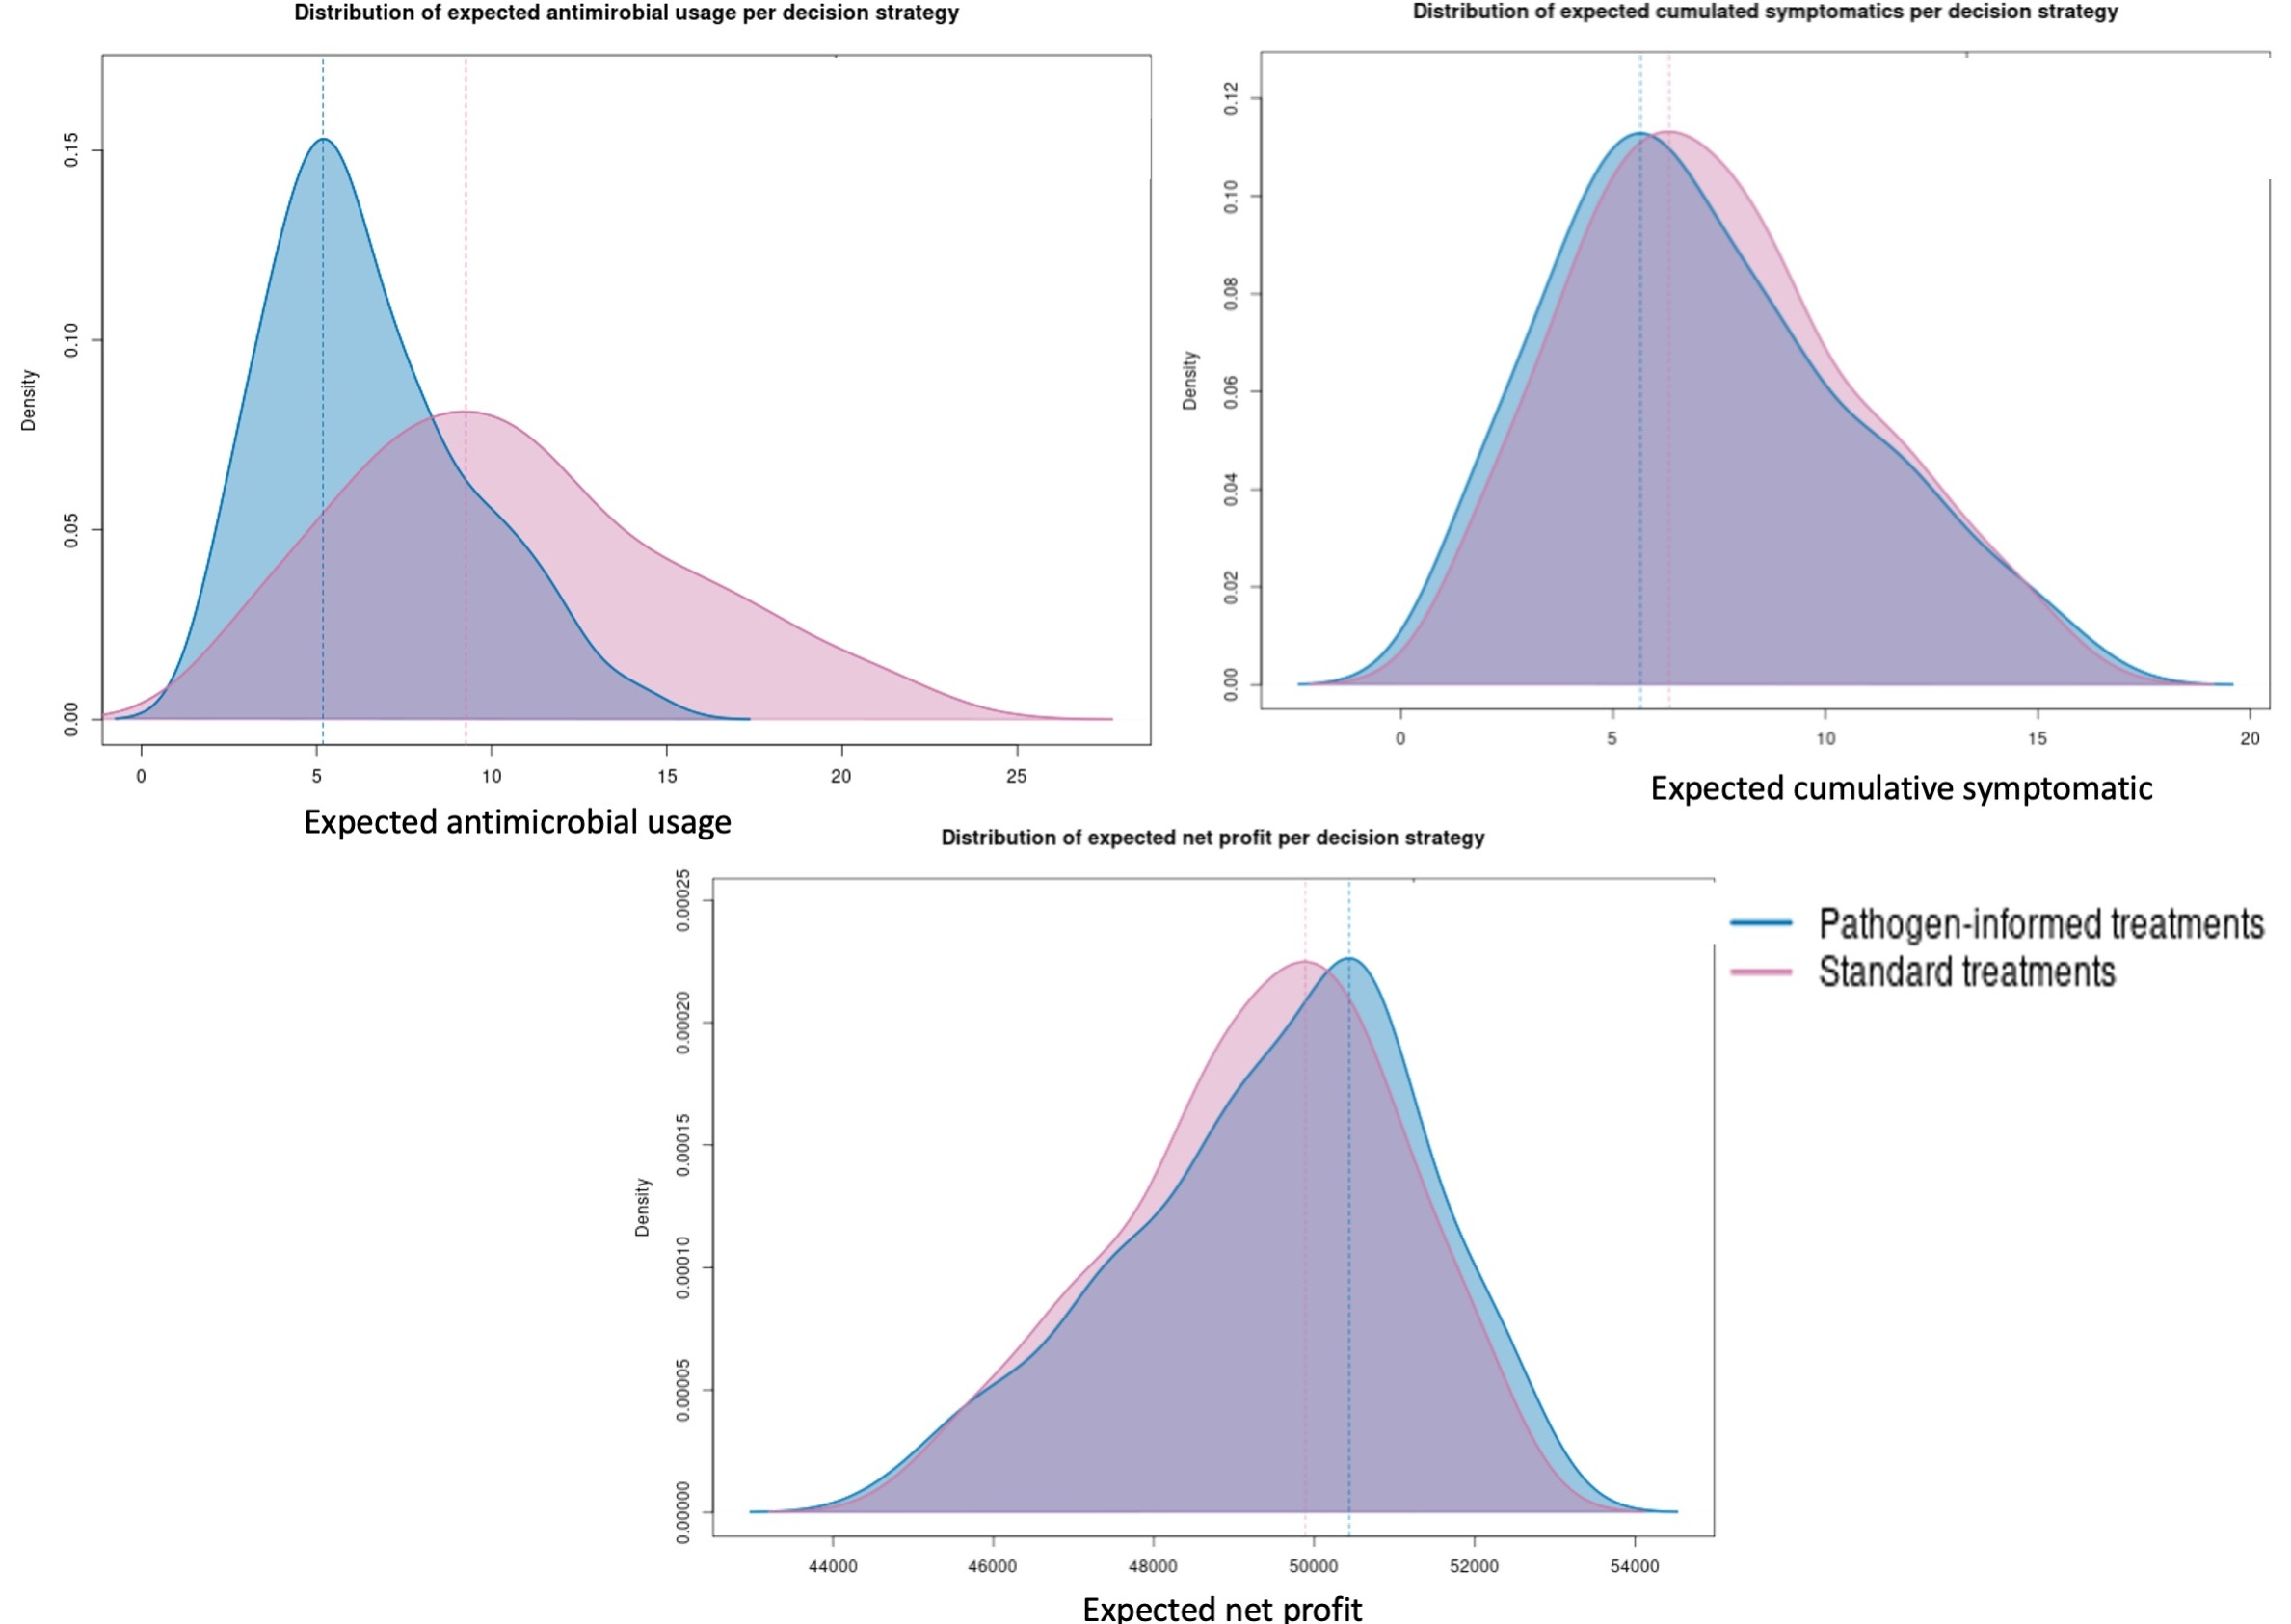
\includegraphics[width=\linewidth]{figures/chap3/expectations.jpg}
  \caption{Pathogen informed treatment decisions versus conventional treatment decisions.}
  \label{fig:chap3-expectation}
\end{figure}

\subsubsection*{Perspectives}

This work bridges theoretical epidemiological modelling with practical decision-making, emphasizing the importance of model distinguishability not only theoretically but as a practical tool for veterinary epidemiology and livestock management. Our approach is broadly applicable to scenarios where pathogen differentiation based solely on observations remains challenging yet essential. In the next chapter, we further explore integrating a real-world observation (sensor-based) for immediate diagnostic insights (deep learning-driven) with longer-term, prognosis-oriented mechanistic epidemiological models, combining these two forms of expertise to generate actionable disease management recommendations.

\subsection{[In French] Résumé grand public}
La gestion efficace des maladies respiratoires bovines (BRD) constitue un enjeu crucial pour la santé animale et pour l’économie des élevages bovins. Ces maladies sont complexes car elles impliquent souvent plusieurs pathogènes différents, notamment des virus comme Orthopneumovirus bovis (BRSV), et des bactéries telles que Mannheimia haemolytica (Mh) ou Mycoplasmopsis bovis (Mb). Chaque pathogène possède ses propres particularités en matière de transmission, de symptômes et de réponse au traitement, rendant leur identification précise essentielle pour une gestion optimale.

Dans ce chapitre, nous avons proposé une approche basée sur la modélisation mécaniste afin d’identifier quel pathogène est à l’origine d’une épidémie, simplement à partir des symptômes observés chez les animaux. Notre méthode utilise des modèles mécanistes spécifiques à chaque pathogène, pour déterminer avec fiabilité l’agent responsable d’une épidémie sur une exploitation. Grâce à des simulations numériques réalistes, nous avons montré que cette identification est possible avec une précision élevée (environ 93\% en moyenne).

Cette identification précise présente des avantages pratiques majeurs pour les éleveurs. Aujourd'hui, faute d’identification fiable, les traitements antibiotiques sont souvent administrés à tous les animaux symptomatiques sans distinction, même si certains souffrent d’infections virales pour lesquelles les antibiotiques sont inefficaces. Cette pratique entraîne une utilisation excessive et inutile des antibiotiques, augmentant le risque de résistance bactérienne, tout en générant des coûts économiques inutiles. Notre étude démontre que l’intégration de ces modèles spécifiques dans une démarche décisionnelle permet une réduction d'environ 44\% de la consommation d’antibiotiques tout en maintenant, voire en augmentant légèrement (~1\%), la rentabilité des exploitations.

Ainsi, ce travail met en évidence l’intérêt concret des modèles mécanistes pour améliorer les décisions pratiques en élevage, réduisant à la fois les coûts économiques et les risques sanitaires liés à une mauvaise utilisation des traitements. Cette approche pourrait s’appliquer à d’autres contextes épidémiologiques où identifier précisément le pathogène à partir de simples observations cliniques reste un défi majeur.


%-----------------------------------
%	SECTION 
%-----------------------------------
\section{Peer-reviewed preprint in bioarxiv, 2025}


    % \input{chapters/chap1-article} # pas besoin de mettre un file appart sauf si j'ai des choses spécifiques à rajouter pour cette partie
    \includepdf[pages=-]{articles/article3.pdf}  % Replace with your actual filename
    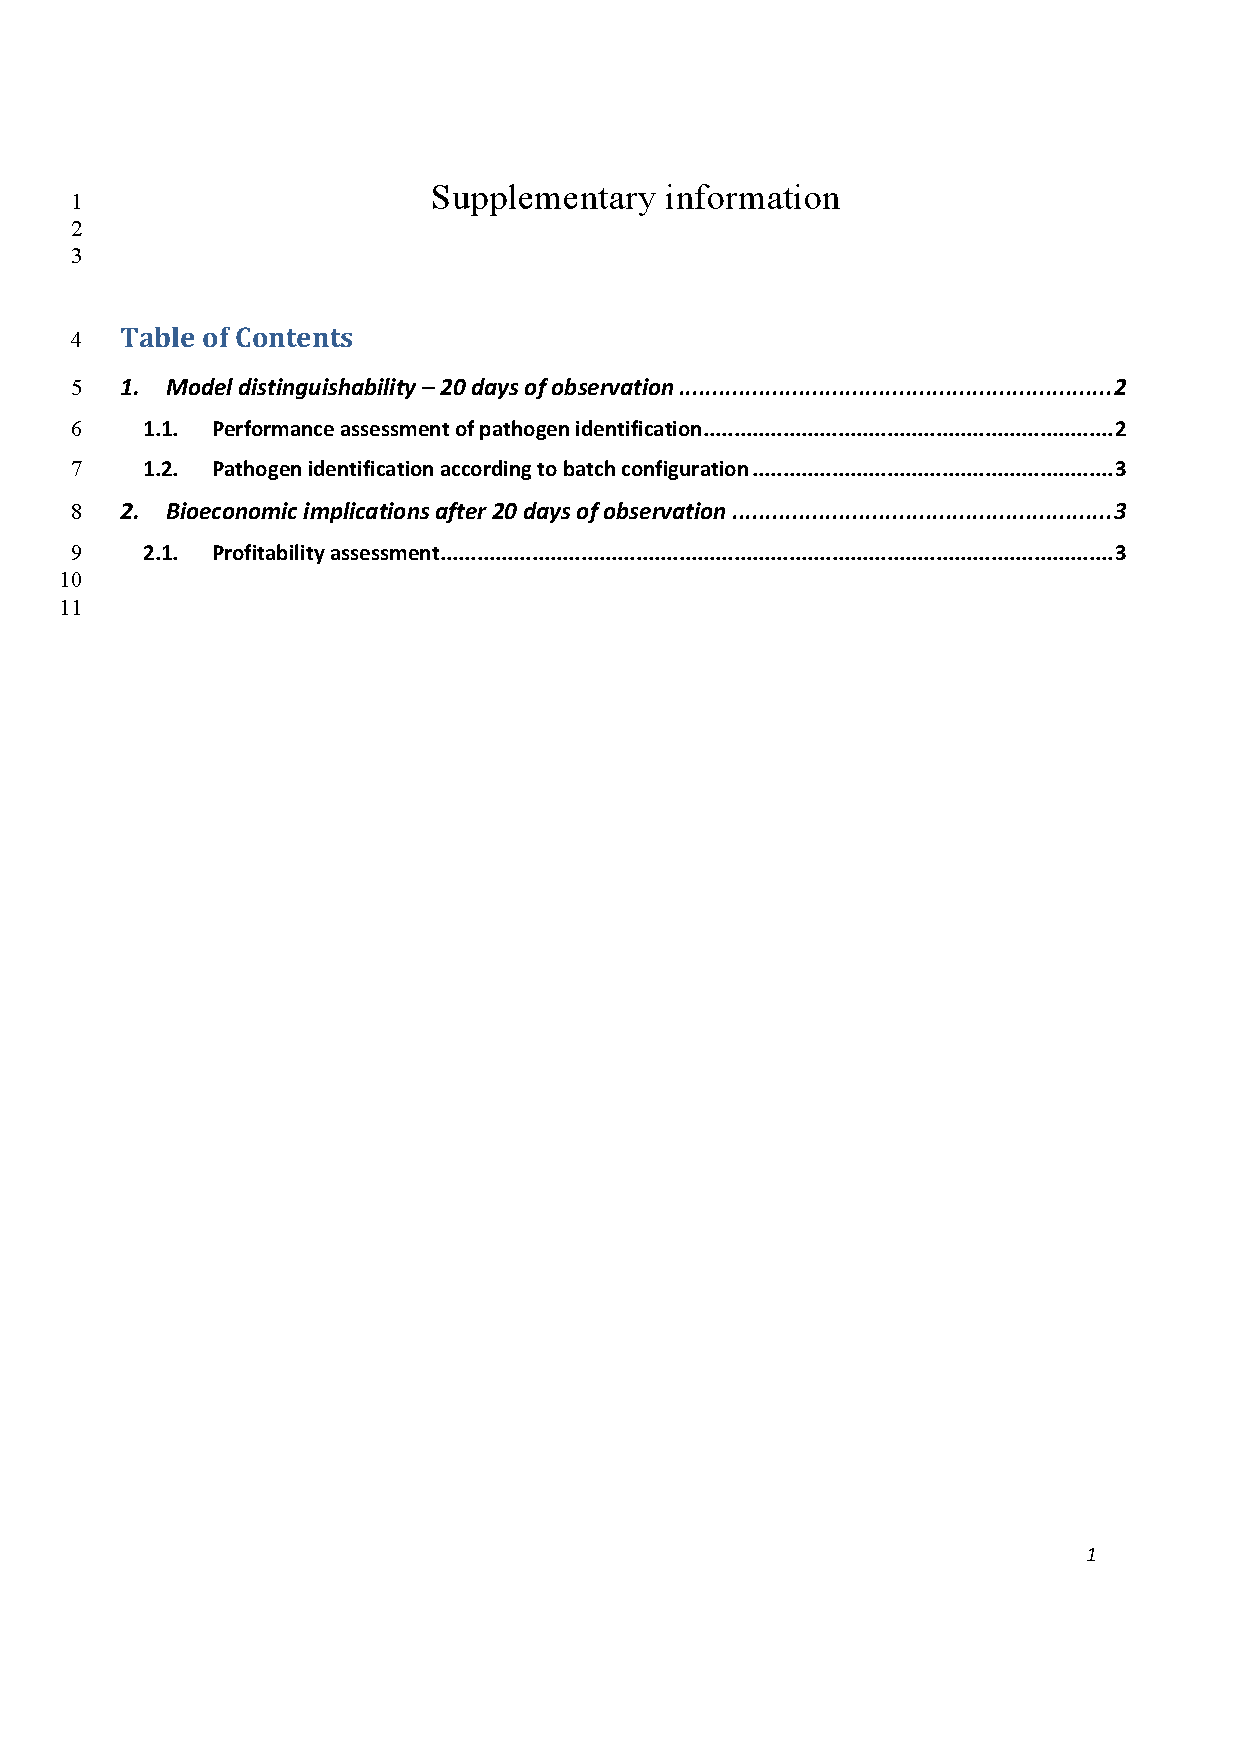
\includepdf[pages=-]{articles/supp-mat3.pdf}
